\documentclass{beamer}
\usepackage[utf8]{inputenc}

\usetheme{Madrid}
\usecolortheme{default}
\usepackage{amsmath,amssymb,amsfonts,amsthm}
\usepackage{txfonts}
\usepackage{tkz-euclide}
\usepackage{listings}
\usepackage{adjustbox}
\usepackage{array}
\usepackage{tabularx}
\usepackage{gvv}
\usepackage{lmodern}
\usepackage{circuitikz}
\usepackage{tikz}
\usepackage{graphicx}

\setbeamertemplate{page number in head/foot}[totalframenumber]

\usepackage{tcolorbox}
\tcbuselibrary{minted,breakable,xparse,skins}



\definecolor{bg}{gray}{0.95}
\DeclareTCBListing{mintedbox}{O{}m!O{}}{%
  breakable=true,
  listing engine=minted,
  listing only,
  minted language=#2,
  minted style=default,
  minted options={%
    linenos,
    gobble=0,
    breaklines=true,
    breakafter=,,
    fontsize=\small,
    numbersep=8pt,
    #1},
  boxsep=0pt,
  left skip=0pt,
  right skip=0pt,
  left=25pt,
  right=0pt,
  top=3pt,
  bottom=3pt,
  arc=5pt,
  leftrule=0pt,
  rightrule=0pt,
  bottomrule=2pt,
  toprule=2pt,
  colback=bg,
  colframe=orange!70,
  enhanced,
  overlay={%
    \begin{tcbclipinterior}
    \fill[orange!20!white] (frame.south west) rectangle ([xshift=20pt]frame.north west);
    \end{tcbclipinterior}},
  #3,
}
\lstset{
    language=C,
    basicstyle=\ttfamily\small,
    keywordstyle=\color{blue},
    stringstyle=\color{orange},
    commentstyle=\color{green!60!black},
    numbers=left,
    numberstyle=\tiny\color{gray},
    breaklines=true,
    showstringspaces=false,
}
%------------------------------------------------------------
%This block of code defines the information to appear in the
%Title page
\title %optional
{1.4.19}
\date{August 28, 2025}
%\subtitle{A short story}

\author % (optional)
{Aditya Appana - EE25BTECH11004}



\begin{document}


\frame{\titlepage}
\begin{frame}{Question}
Find the acute angle between the planes $ \vec{r} \cdot (\hat{i} - 2\hat{j} - 2\hat{k} ) = 1$ and  $ \vec{r} \cdot (3\hat{i} - 6\hat{j} + 2\hat{k})=0$.

\end{frame}
\begin{frame}{allowframebreaks}
\frametitle{Given Information}

    \centering
    
    \label{tab:parameters}
    
    
    Let vector $\vec{n_1}$ be: \begin{align}
    \myvec{1\\-2\\-2}
    \end{align}
    

    Let vector $\vec{n_2}$ be: \begin{align}\myvec{3\\-6\\2}\end{align}
    \label{0.2}

   
\end{frame}


\begin{frame}{Formula}
The formula to calculate the angle between the two planes is
\begin{align}
\theta = \frac{\pi}{2} - \cos^{-1}\brak{\frac{\vec{n_1}^T\vec{n_2}}{|\vec{n_1}||\vec{n_2}|}}
= \sin^{-1}\brak{\frac{\vec{n_1}^T\vec{n_2}}{|\vec{n_1}||\vec{n_2}|}}
\end{align}



\end{frame}

\begin{frame}{allowframebreaks}
\frametitle{Solution}
Substituting $\mathbf{P, Q}$ in this formula :
\begin{align*}
= \sin^{-1}\brak{\frac{\myvec{1\\-2\\-2}^T\myvec{3\\-6\\2}}{|\myvec{1\\-2\\-2}||\myvec{3\\-6\\2}|}}
= \sin^{-1}\brak{\frac{19}{|3||7|}}
= \sin^{-1}\brak{\frac{11}{21}}
\end{align*}
\centering
This is 31.58906757233914°
\end{frame}




\begin{frame}[fragile]
    \frametitle{Python Code}
    \begin{lstlisting}
import numpy as np
import matplotlib.pyplot as plt
import sys
import numpy.linalg as LA
import math

vec1 = np.array([1,-2,-2])
vec2 = np.array([3,-6,2])

dot_product = vec1@vec2

norm1 = np.linalg.norm(vec1)
norm2 = np.linalg.norm(vec2)

cos = dot_product/(norm1*norm2)
angle = math.asin(cos)
print(angle*180/3.1415)

\end{lstlisting}
\end{frame}

\begin{frame}[fragile]
    \frametitle{Python Code}

    \begin{lstlisting}
fig = plt.figure()
ax = fig.add_subplot(111, projection='3d')

x = np.linspace(-10, 10, 20)
y = np.linspace(-10, 10, 20)
X, Y = np.meshgrid(x, y)

Z = (X-2*Y- 1)/2
z1 = (6*Y - 3*X)/2

ax.plot_surface(X, Y, Z, alpha=1, cmap='Blues')
ax.plot_surface(X, Y, z1, alpha=1, cmap='Oranges')

ax.set_xlabel('X axis')
ax.set_ylabel('Y axis')
ax.set_zlabel('Z axis')
ax.set_title('Plot of the planes')
plt.show()

    \end{lstlisting}
\end{frame}


\begin{frame}{Plot 1}
\begin{figure}
    \centering
    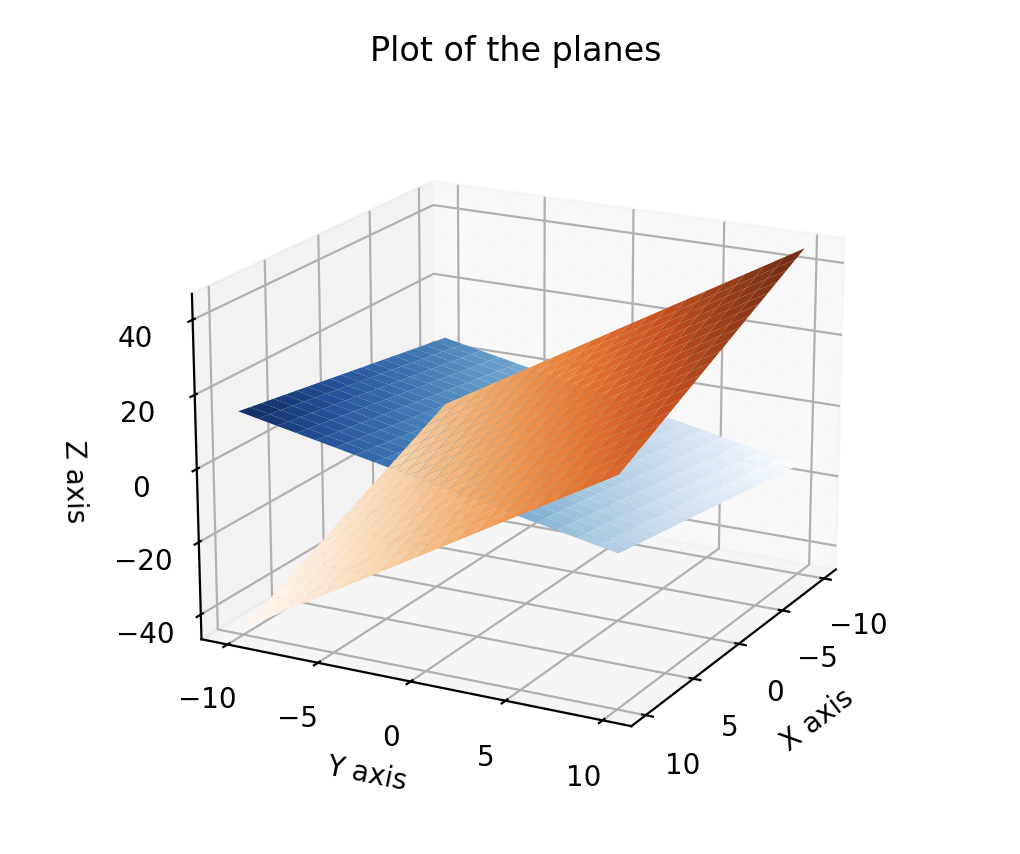
\includegraphics[width=0.8\columnwidth]{Figs/Figure_3.2.png}
    \caption{Plot}
    \label{fig:placeholder}
\end{figure}
\end{frame}

\begin{frame}{Plot 2}
\begin{figure}
    \centering
    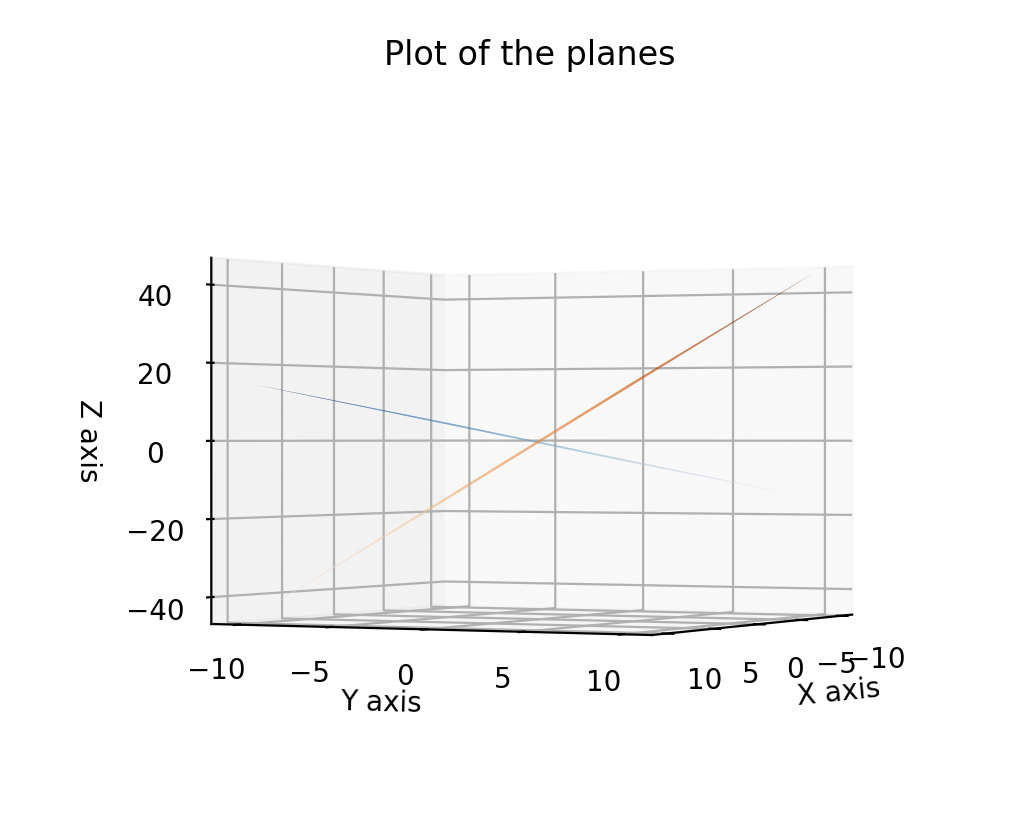
\includegraphics[width=0.8\columnwidth]{Figs/Figure_3.1.png}
    \caption{Plot}
    \label{fig:placeholder}
\end{figure}
\end{frame}

\begin{frame}[fragile]
\frametitle{C Code}
\begin{lstlisting}
#include<stdio.h>
#include<math.h>


float anglefinder(float x1, float y1, float z1, float x2, float y2, float z2){

float dot_product;
float mod1;
float mod2;
float cosval;
float angle;

dot_product = x1*x2 + y1*y2 + z1*z2;



\end{lstlisting}

\end{frame}

\begin{frame}[fragile]
\frametitle{C Code}
\begin{lstlisting}
mod1 = pow(x1,2) + pow(y1,2) + pow(z1,2);    
mod2 = pow(x2,2) + pow(y2,2) + pow(z2,2);
    
mod1 = sqrt(mod1);
mod2 = sqrt(mod2);
   
cosval = dot_product/(mod1 * mod2);

angle= asin(cosval);

return angle;
}

\end{lstlisting}

\end{frame}


\begin{frame}[fragile]
\frametitle{Python and C Code}

\begin{lstlisting}
import numpy as np
import matplotlib.pyplot as plt
import sys
import ctypes

c_lib=ctypes.CDLL('./3c.so')

c_lib.anglefinder.argtypes = [ctypes.c_float, ctypes.c_float,ctypes.c_float, ctypes.c_float, ctypes.c_float, ctypes.c_float]
c_lib.anglefinder.restype = ctypes.c_float



\end{lstlisting}

\end{frame}

\begin{frame}[fragile]
\frametitle{Python and C Code}
\begin{lstlisting}

v1 = np.array([1,2,-2])
v2 = np.array([3,-6,2])

angle = c_lib.anglefinder(
    ctypes.c_float(v1[0]),
    ctypes.c_float(v1[1]), 
    ctypes.c_float(v1[2]),
    ctypes.c_float(v2[0]), 
    ctypes.c_float(v2[1]),
    ctypes.c_float(v2[2])
)

print(angle*180/3.1415)

\end{lstlisting}

\end{frame}

\begin{frame}[fragile]
\frametitle{Python and C Code}

\begin{lstlisting}
c_lib=ctypes.CDLL('./main.so')

# Define the argument types for the x function
c_lib.xfinder.argtypes = [ctypes.c_float, ctypes.c_float,ctypes.c_float, ctypes.c_float]
# Define the return type of the x function
c_lib.xfinder.restype = ctypes.c_float
# --- Define Points and Calculate 'm' using C function ---

v1 = np.array([7,6])
v2 = np.array([3,4])

xcoord = c_lib.xfinder(
    ctypes.c_float(v1[0]),
    ctypes.c_float(v1[1]), 
    ctypes.c_float(v2[0]), 
    ctypes.c_float(v2[1])
)
\end{lstlisting}

\end{frame}

\begin{frame}[fragile]
    \frametitle{Python Code}

    \begin{lstlisting}
fig = plt.figure()
ax = fig.add_subplot(111, projection='3d')

x = np.linspace(-10, 10, 20)
y = np.linspace(-10, 10, 20)
X, Y = np.meshgrid(x, y)

Z = (X-2*Y- 1)/2
z1 = (6*Y - 3*X)/2

ax.plot_surface(X, Y, Z, alpha=1, cmap='Blues')
ax.plot_surface(X, Y, z1, alpha=1, cmap='Oranges')

ax.set_xlabel('X axis')
ax.set_ylabel('Y axis')
ax.set_zlabel('Z axis')
ax.set_title('Plot of the planes')
plt.show()

    \end{lstlisting}
\end{frame}


\begin{frame}{Plot 1}
\begin{figure}
    \centering
    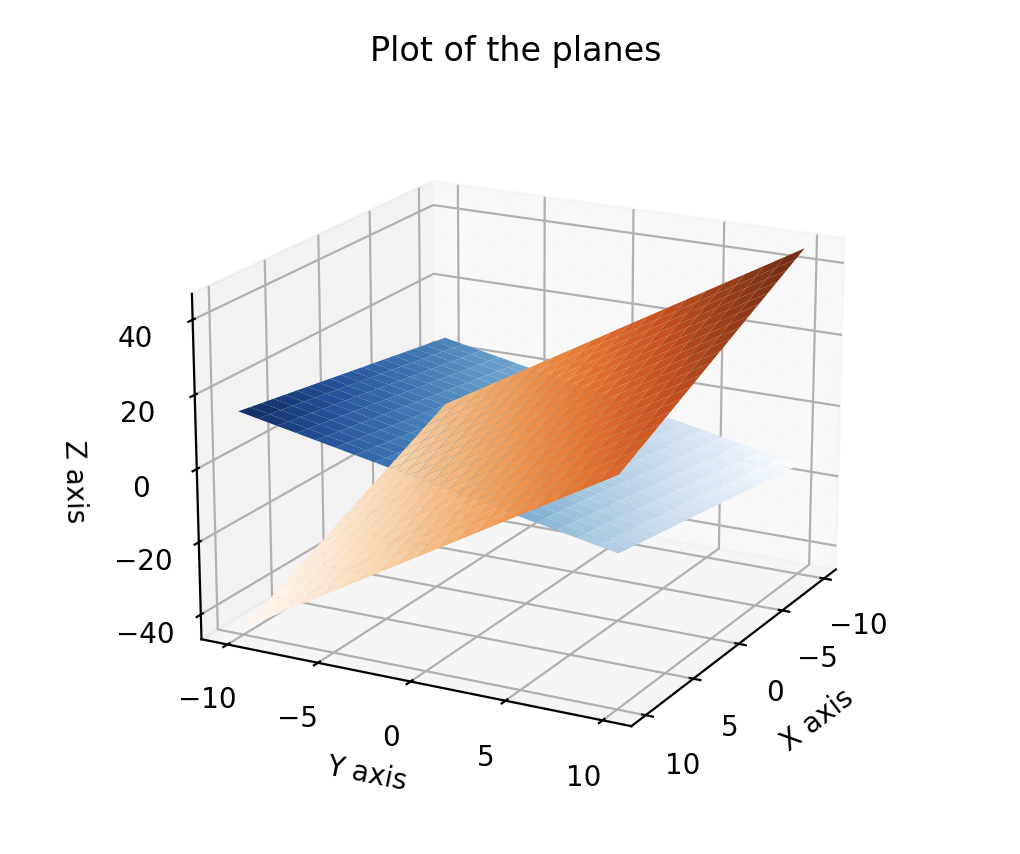
\includegraphics[width=0.8\columnwidth]{Figs/Figure_3.2.png}
    \caption{Plot}
    \label{fig:placeholder}
\end{figure}
\end{frame}

\begin{frame}{Plot 2}
\begin{figure}
    \centering
    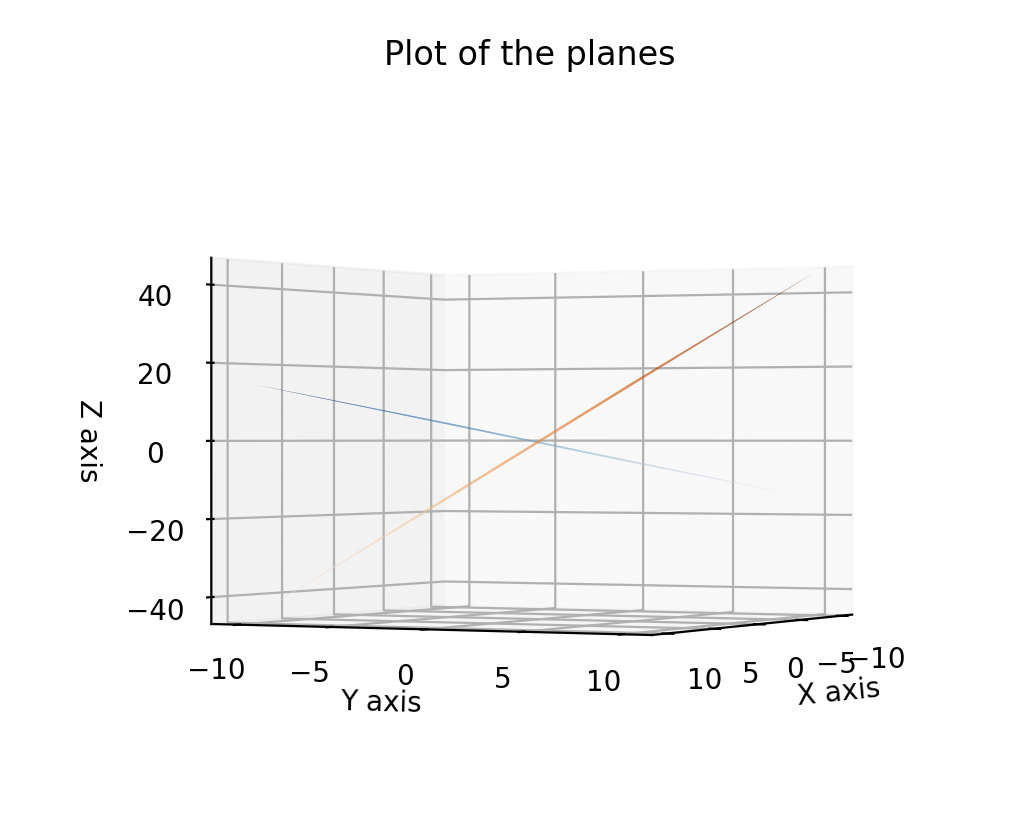
\includegraphics[width=0.8\columnwidth]{Figs/Figure_3.1.png}
    \caption{Plot}
    \label{fig:placeholder}
\end{figure}
\end{frame}

\end{document}